\documentclass [bachelor,a4paper,11pt,oneside,deutsch,todo,nolistofalgorithms,webreferences,noglossary,listoflistings,acronym]{INSOthesis}
% change encoding in the document
%\inputencoding{utf8} % default
%\inputencoding{latin1} % for windows

\thesistitle{Unterstützung der IT–Sicherheit von VoIP–Infrastrukturen durch die Verwendung spezialisierter VoIP–Firewalls}
%\thesisshorttitle{Shorttitle of the Thesis}
%\thesissubtitle{Optional Subtitle} % optional
\thesisdate{\today}

% all titles and designations have to be gender-related!
%\thesistype{Diplomarbeit}{Master's Thesis}
%\thesisdegree{Diplom-Ingenieurin}{Diplom-Ingenieurin}
\thesistype{Bakkalaureatsarbeit}{Bachelor's Thesis}
\thesisdegree{Bakk.tech.}{Bakk.tech.}
\thesiscurriculum{Wirtschaftsinformatik}{Business Informatics} % your study
\thesisauthor{Philipp Schaden} % your name
\thesisauthoraddress{Aschau 93, 7432 Oberschützen} % your address
\thesismatrikelno{0626698} % your registration number

% advisor
%\thesisauthorpreamble {Verfasser}
\thesisadvisorpreamble {Betreuung}
\thesisadvisorone {Thomas Grechenig}
\thesisadvisortwo {Florian Fankhauser}
%\thesisadvisorthree {Vorname Nachname

% Bibliographie file
\bibliography{bibliography/references}

\hypersetup{
  %colorlinks=false % enable and disable frames arround links
}

%%%%%%%%%%%%%%%%%%%%%%%%%%%%%%%%%%%%%%%%%%%%%
%
% Can be used to add additional informations
% 
%%%%%%%%%%%%%%%%%%%%%%%%%%%%%%%%%%%%%%%%%%%%%
% \AfterTitlePages{}
% \AfterDeclaration{}
% \AfterAcknowledgements{}
% \AfterAbstract{}
% \AfterListOfFigures{}
% \AfterListOfTables{}
% \AfterAbbreviations{}
% \AfterBibliography{}

\renewcommand\afterchapternum{\hspace{1em}}
\begin{document}

\maketitle

%%%%%%%%%%%%%%%%%%%%%%%%%%%%%%%%%%%%%%%%%
%%%   CONTENTS    %%%%%%%%%%%%%%%%%%%%%%%
%%%%%%%%%%%%%%%%%%%%%%%%%%%%%%%%%%%%%%%%%
%\section{General Information}

This document is intended as a template and guideline and should support the author in the course of doing the master's thesis.
Assessment criteria comprise the quality of the theoretical and/or practical work as well as structure, content and wording of the written master's thesis. Careful attention should be given to the basics of scientific work (e.g., correct citation).\footnote{Sample Footnote}

\section{Organizational Issues}

A master's thesis at the Faculty of Informatics has to be finished within six months. During this period regular meetings between the advisor(s) and the author have to take place.
In addition, the following milestones have to be fulfilled:
\begin{enumerate}
  \item  Within one month after having fixed the topic of the thesis the master's thesis proposal has to be prepared and must be accepted by the advisor(s). The master's thesis proposal must follow the respective template of the dean of academic affairs. Thereafter the proposal has to be applied for at the deanery. The necessary forms may be found on the web site of the Faculty of Informatics. \url{http://www.informatik.tuwien.ac.at/dekanat/formulare.html}
  \item  Accompanied with the master's thesis proposal, the structure of the thesis in terms of a table of contents has to be provided.
  \item Then, the first talk has to be given at the so-called ``Seminar for Master Students''. The slides have to be discussed with the advisor(s) one week in advance. Attendance of the ``Seminar for Master Students'' is compulsory and offers the opportunity to discuss arising problems among other master students.
  \item At the latest five months after the beginning, a provisional final version of the thesis has to be handed over to the advisor(s).  
  \item As soon as the provisional final version exists, a first poster draft has to be made. The making of a poster is a compulsory part of the ``Seminar for Master Students'' for all master studies at the Faculty of Informatics. Drafts and design guidelines can be found at \url{http://www.informatik.tuwien.ac.at/studium/richtlinien}.
  \item After having consulted the advisor(s) the second talk has to be held at the ``Seminar for Master Students''.
  \item At the latest six months after the beginning, the corrected version of the master's thesis and the poster have to be handed over to the advisor(s).
  \item After completion the master's thesis has to be presented at the ``epilog''. For detailed information on the epilog see: \\ \url{http://www.informatik.tuwien.ac.at/studium/epilog}
\end{enumerate}

\section{Structure of the Master's Thesis}

If the curriculum regulates the language of the master's thesis to be English (like for ``Business Informatics''), the thesis has to be written in English. Otherwise, the master's thesis may be written in English or in German. The structure of the thesis is predetermined.
The table of contents is followed by the introduction and the main part, which can vary according to the content. The master's thesis ends with the bibliography (compulsory) and the appendix (optional).

\begin{itemize}
  \item	Cover page
  \item Acknowledgements
  \item Abstract of the thesis in English and German
  \item Table of contents
  \item Introduction
  	\begin{itemize}
  		\item motivation
  		\item problem statement (which problem should be solved?)
  		\item aim of the work
  		\item methodological approach
  		\item structure of the work
  	\end{itemize}
  \item State of the art / analysis of existing approaches
  	\begin{itemize}
  		\item literature studies
  		\item analysis
  		\item comparison and summary of existing approaches
  	\end{itemize}
  \item Methodology
  	\begin{itemize}
  		\item used concepts
  		\item methods and/or models
  		\item languages
  		\item design methods
  		\item data models
  		\item analysis methods
  		\item formalisms
  	\end{itemize}
  \item Suggested solution/implementation
  \item Critical reflection
  	\begin{itemize}
  		\item comparison with related work
  		\item discussion of open issues
  	\end{itemize}
  \item Summary and future work
  \item Appendix: source code, data models, \dots
  \item Bibliography
\end{itemize}


%%%%%%%%%%%%%%%%%%%%%%%%%%%%%%%%%%%%%%%%%%%%%%%%%%%%%%%%%%%%%%%%%%%%%%%%%
\chapter{Grundlagen}
\label{sec:fundamentals}
%%%%%%%%%%%%%%%%%%%%%%%%%%%%%%%%%%%%%%%%%%%%%%%%%%%%%%%%%%%%%%%%%%%%%%%%

In diesem Kapitel werden die theoretischen Grundlagen und alle in der Arbeit verwendeten und für das Verständnis relevante Begriffe erläutert. Kapitelnamen spezifizieren, anpassen an die Fragestellung der Arbeit.

Nach dem Lesen dieses Kapitels sollten folgende Punkte klar dargestellt sein:
\begin{itemize}
	\item Beschreibung der relevanten theoretischen Grundlagen für die Behandlung der Fragestellung
	\item Detaillierte Beschreibung ggf. vorhandener relevanter Spezifika des Anwendungsbereichs, in dem das Problem gelöst wird
	\item Detaillierte Beschreibung relevanter Spezifika eingesetzter Technologien
	\item Analyse bestehender Ansätze/ Vorarbeiten: Literaturstudium, Analyse, Vergleich und Zusammenfassung bestehender Ansätze. 
\end{itemize}

Gerade im Bereich der Grundlagen wird viel Literatur zitiert -- Details zum Zitieren finden Sie im Kapitel \ref{sec:references}. Da keine Diplomarbeit so innovativ ist, dass sie nicht auf vorhandenes Wissen aufbaut und in ein entsprechendes Forschungsumfeld eingebettet ist, kommt an dieser Stelle der Literaturrecherche eine besondere Bedeutung zu. Als Daumenregel gilt, dass der aktuelle Stand der Wissenschaft in der Informatik üblicherweise durch Publikationen v.a. der letzten 2 – 4 Jahre repräsentiert wird. 

Beispielhaft einleitender Text an dieser Stelle:\\
Dieses Kapitel stellt Konzepte der Informationstheorie vor und liefert theoretische Grundlagen zu verdeckten Kanälen. Die verdeckte Kommunikation wird mit den verwandten Techniken der Steganographie und Kryptographie verglichen. Außerdem werden ein einfaches Fehlerkorrekturverfahren sowie die Grundlagen des HTTP-Protokolls beschrieben.

%=======================================================================
\section{Aktueller Stand der Technik}
%=======================================================================

In diesem Kapitel wird ein Überblick über bereits existierende Lösungen für die Problemstellung bzw. verwandte Problemstellungen gegeben. Dabei ist eine Klassifizierung der existierenden Lösungen empfehlenswert. Eine Analyse der Lösungen, nach Kriterien sortiert, sollte insbesondere auch die Defizite der existierenden Lösungen erläutern und damit insbesondere auch eine Begründung liefern, warum diese Lösungen für die Problemstellung der Arbeit nicht herangezogen werden können.

%-----------------------------------------------------------------------
\subsection{Unterkapitel}
%-----------------------------------------------------------------------

Bei der Verwendung von Gliederungsebenen gibt es Folgendes zu beachten:
\begin{itemize}
	\item Es sollten nicht mehr als 3 Gliederungstiefen nummeriert werden.
	\item Unterkapitel sind nur dann sinnvoll, wenn es auch mehrere Untergliederungen gibt. Ein Kapitel 2.1.1 sollte somit nur dann verwendet werden, wenn es auch 2.1.2 gibt.
	\item Oft ist es einfacher und besser verständlich, Aufzählungen als Text zu formulieren und somit weitere Gliederungsstufen zu vermeiden.
\end{itemize}

%-----------------------------------------------------------------------
\subsection{Abbildungen}
\label{sec:abbildungen}
%-----------------------------------------------------------------------

Beschreibungen zu Abbildungen und Tabellen stehen unter dem Bild. Jede Abbildung muss im Fließtext referenziert werden. In \LaTeX besitzen Abbildungen typischerweise Labels, welche zum referenzieren verwendet werden. Zudem plaziert \LaTeX die Abbildungen an geeigneten Stellen, was meistens auch wünschenswert ist. Falls das nicht gewünscht wird, kann es durch Optionen beeinflusst werden.

Abbildung \ref{fig:xxx} verdeutlicht  \dots\\
(siehe Abbildung \verb|\ref{<label>}|)

\begin{figure}
	\centering
	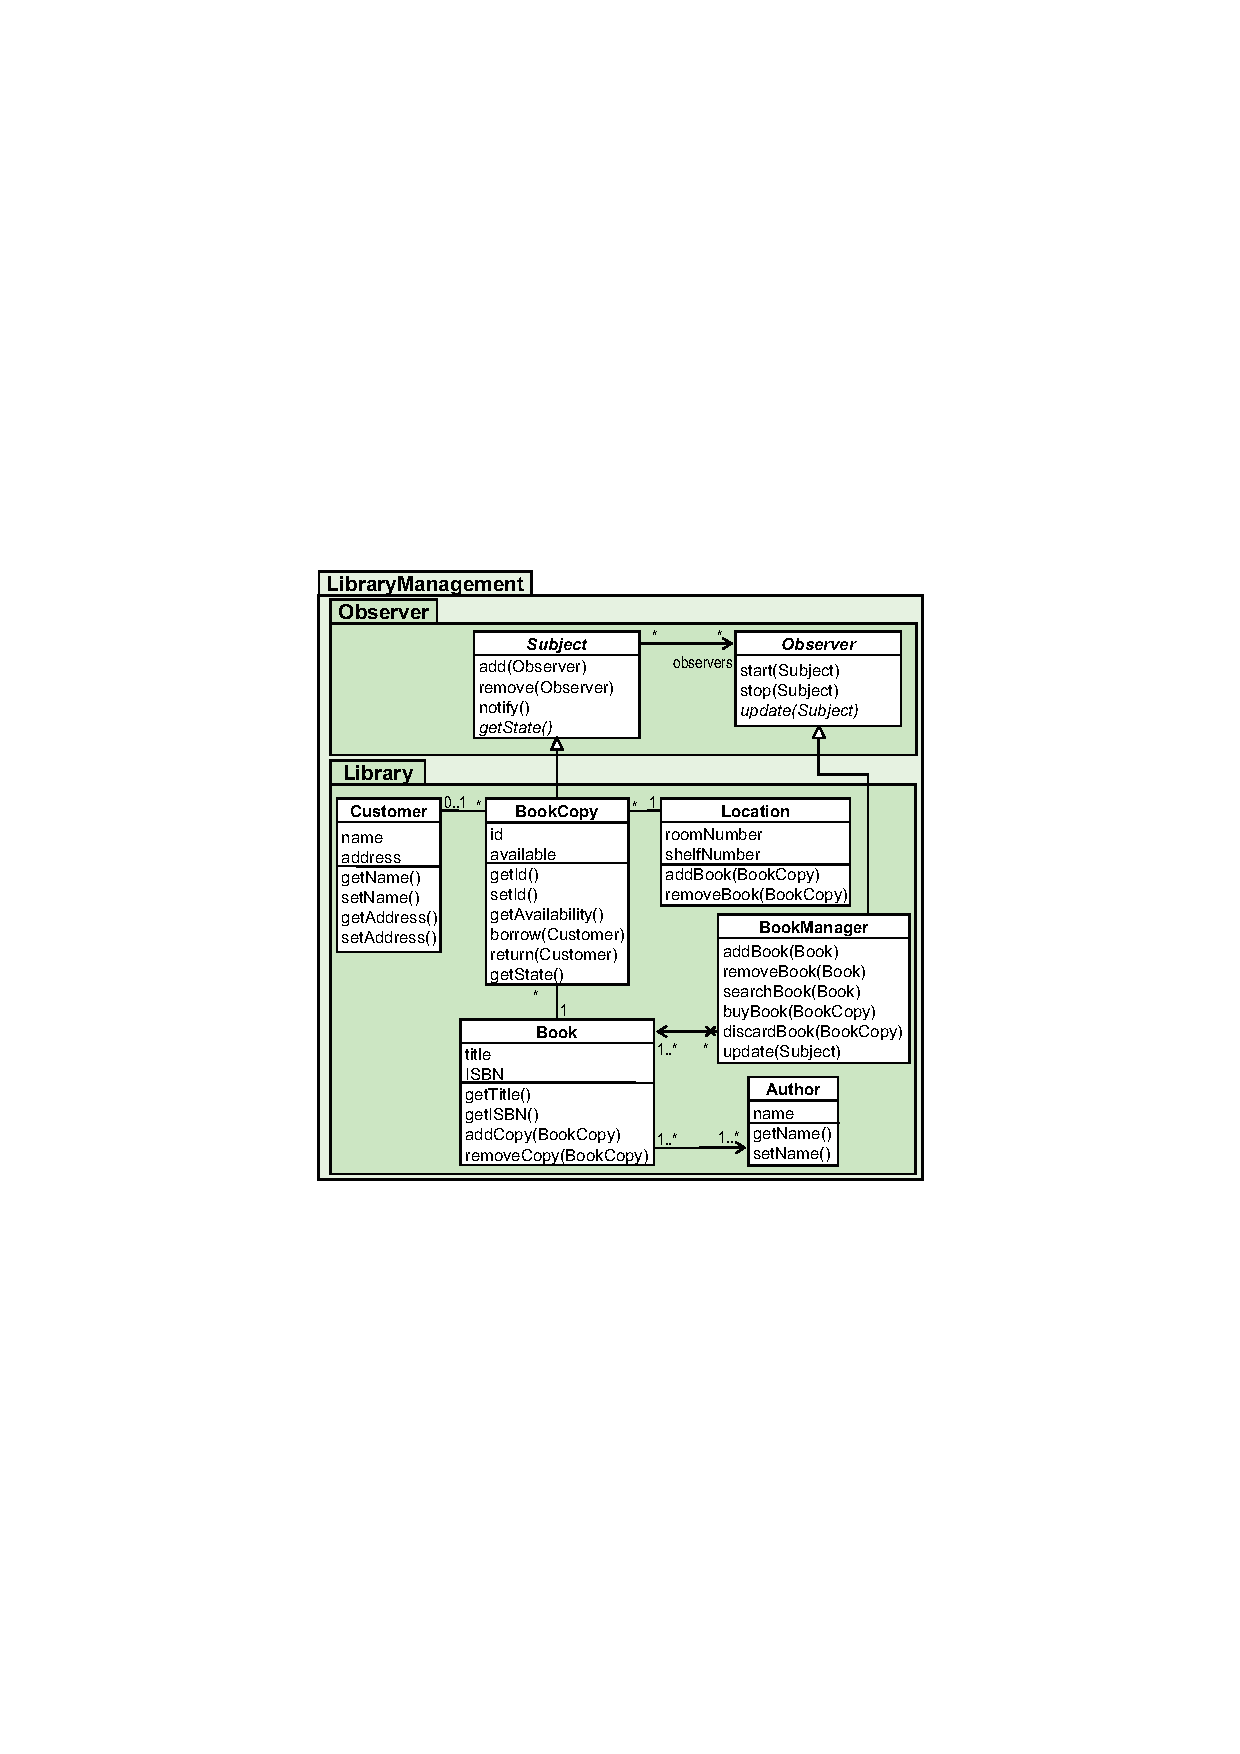
\includegraphics[width=0.4\linewidth]{figures/figure1}
	\caption{xxx (Quelle zitieren, wenn nicht selbst erstellt)}
	\label{fig:xxx}
\end{figure}

%-----------------------------------------------------------------------
\subsection{Tabellen}
%-----------------------------------------------------------------------

Jede Tabelle muss im Fließtext referenziertw werden. Für Tabellen gelten die selben Regeln, wie für Abbildungen (siehe dazu Abschnitt \ref{sec:abbildungen}).

Eine Beispiel einer Tabelle ist in Tabelle \ref{tab:xxx} zu finden:
\begin{table}
	\centering
	\begin{tabular}{| >{\bfseries}l | c | r | }
		\hline
			\rowcolor{orange} \bfseries Linksbündig & \bfseries Zentriert & \bfseries Rechtsbündig \\
		\hline
		\hline
			Zeile 1 & xxx & xxx \\\hline
			Zeile 2 & xxx & \dots \\\hline
			\multirow{2}{*}{Zeile3}
			& xxx & xxx \\\cline{2-3}
			& xxx & xxx \\\hline
		\hline
			\multicolumn{3}{| c |}{xxx} \\\hline
	\end{tabular}
	\caption{xxx (Quelle angeben)}
	\label{tab:xxx}
\end{table}

Grundsätzlich wird empfohlen Tabllen so simple wie möglich zu halten und spielereien wie Farbe zu unterlassen.
%%%%%%%%%%%%%%%%%%%%%%%%%%%%%%%%%%%%%%%%%%%%%%%%%%%%%%%%%%%%%%%%%%%%%%%%%
\chapter{Konkrete Problemstellung -- Umfeldbeschreibung}
\label{sec:problemdescription}
%%%%%%%%%%%%%%%%%%%%%%%%%%%%%%%%%%%%%%%%%%%%%%%%%%%%%%%%%%%%%%%%%%%%%%%%

In diesem Kapitel wird die eigentliche Problemlösung in einem oder mehreren Unterkapiteln ausgeführt. Die Strukturierung dieser Kapitel ist naturgemäß sehr stark von der konkreten Aufgabenstellung abhängig. Der Name dieses Kapitels ist anzupassen, z.B. Umfeldbeschreibung -- Fallbeispiel \dots, konkreter schreiben je nach Art Diplomarbeit/Fragestellung. Nachfolgend einige Beispiele für unterschiedliche Arten von Diplomarbeiten. 

Bei einer Software-Entwicklungsarbeit bieten sich folgende Unterkapitel an:
\begin{itemize}
	\item Im Kapitel \enquote{Design} sollte die konzeptionelle Lösung vorgestellt, diskutiert und begründet werden. Das Ergebnis dieses Kapitels könnte beispielsweise eine Protokoll-Architektur sein.
	\item Im Kapitel \enquote{Modelle} erfolgt üblicherweise das Feindesign. In diesem Kapitel könnten beispielsweise einzelne Protokolle bzw. Algorithmen aus der vorher definierten Protokoll-Architektur eingeführt und diskutiert werden. Achtung: Generell darauf achten, bei der eingangs erläuterten Notation zu bleiben und nicht Synonyme zu verwenden, verwirrt den Leser.
	\item Das Kapitel \enquote{Implementierung} sollte sich dann vorwiegend mit den Details der Umsetzung befassen. In diesem Kapitel sollte nur im Ausnahmefall exemplarisch Quellcode vorgesehen werden. Vielmehr sollten alle Probleme, die bei der Realisierung aufgetreten sind, dokumentiert, interpretiert und die Lösung erläutert werden.
\end{itemize}

Bei einer Arbeit zu einem abstrakteren Thema, bei dem ein oder mehrere Fallbeispiele aus der industriellen Praxis bearbeitet werden, bieten sich folgende Unterkapitel an:
\begin{itemize}
	\item Im Unterkapitel \enquote{Analyse der Problemstellung} wird die konkrete Problemstellung (die Situation im betrachteten Unternehmen) der Fallbeispiele beschrieben. Das Ergebnis dieses Kapitels könnte eine schematische Netzwerk- oder Applikationsarchitektur sein.
	\item Im Unterkapitel \enquote{Fallbeispiel} sollte sich (analog zur Implementierung in der Software-Entwicklung) mit den konkreten Details der Umsetzung befassen. Hier wird dargelegt, wie das zuvor identifizierte Lösungsschema konkret zur Anwendung gelangen kann bzw. welche Probleme während des Umsetzungsprojekts aufgetreten sind.
\end{itemize}

Bei einer Arbeit, deren Grundlage eine Auswahl eines Softwaresystems ist, bieten sich folgende Unterkapitel an:
\begin{itemize}
	\item IST-Analyse
	\item Hardware und Softwareausstattung
	\item Beschreibung der Geschäftsprozesse
	\item Schwachstellenanalyse des Unternehmens
	\item SOLL-Konzeption
	\item Auswahlverfahren möglicher verfügbarer Systeme -- Kriterienkatalog
	\item Einführung des neuen Systems
\end{itemize}

Bei einer Arbeit, deren Fokus auf der Durchführung und Auswertung von Fragebögen liegt, bieten sich folgende Unterkapitel an:
\begin{itemize}
	\item Im Kapitel \enquote{Problemstellung und Fragebogendesign} wird die fachliche Problemstellung detailliert erläutert und der Inhalt des Fragebogens in Bezug zur Problemstellung dargestellt.
	\item Im Kapitel \enquote{Befragungsmethode} werden die Untersuchungsobjekte (z.B. Praktische Ärzte), die Grundgesamtheit (Anzahl praktische Ärzte in Venezuela), Stichprobengesamtheit und das Verfahren zur Stichprobenziehung und das Erhebungsverfahren (Verteilung und Rücklauf der Fragebögen) beschrieben.
	\item Im Kapitel \enquote{Auswertungsmethode} werden die möglichen Auswertungsmethoden aufgelistet und ggf. begründet die ausgewählte Methode beschrieben.
	\item Im Kapitel \enquote{Befragungsdurchführung} wird die Untersuchungsdurchführung (z.B. Zeit, Ort der Befragung, Zeitraum der gesamten Befragung, besondere für das Untersuchungsergebnis oder zukünftige Forschungsarbeiten relevante Vorkommnisse etc.) dargestellt.
\end{itemize}

Hier intensive Rücksprache mit Ihren jeweiligen Fachbetreuern halten, mehrere Diplomarbeiten der Fakultät zu diesem Themenbereich durchsehen. Unabhängig vom Typ der Diplomarbeit werden im nachfolgenden Kapitel die konkreten Ergebnisse beschrieben.
%%%%%%%%%%%%%%%%%%%%%%%%%%%%%%%%%%%%%%%%%%%%%%%%%%%%%%%%%%%%%%%%%%%%%%%%%
\chapter{Diskussion}
\label{sec:discussion}
%%%%%%%%%%%%%%%%%%%%%%%%%%%%%%%%%%%%%%%%%%%%%%%%%%%%%%%%%%%%%%%%%%%%%%%%

Den akademischen Wert der Arbeit hervorheben, Vergleich mit verwandten Arbeiten: In welchem Verhältnis stehen die Ergebnisse der Diplomarbeit zu den Ergebnissen anderer Studien? Wo gibt es Unterschiede, wo Gemeinsamkeiten? Warum?

Diskussion offener Punkte, Darstellen der Stärken und Schwächen der vorliegenden Ergebnisse.

%%%%%%%%%%%%%%%%%%%%%%%%%%%%%%%%%%%%%%%%%
\chapter{Einleitung}
\label{ch:ch1}
%%%%%%%%%%%%%%%%%%%%%%%%%%%%%%%%%%%%%%%%%
\begin{section}{Problemstellung}
\begin{subsection}{Allgemeine Problemstellung}
Voice Over Internet Protocol (kurz VoIP) ist eine sehr stark wachsende und häufig verwendete Technologie. Insbesondere in großen – aber auch mittelgroßen - Unternehmen findet diese Kommunikationsart Anklang.
Durch diesen hohen Verbreitungsgrad sind viele Sicherheitsprobleme entstanden.
Einige solcher Probleme werden im Zuge dieser Arbeit näher beschrieben.
\\
In dieser wissenschaftlichen Arbeit werden daher die Sicherheit in VoIP-Netzwerken erörtert und die Absicherungsmöglichkeiten mittels einer speziellen VoIP-Firewall ergründet bzw. Sicherheitslücken und Sicherheitsrisiken aufgezeigt.
\end{subsection}
\begin{subsection}{Detaillierte Problemstellung}
Im Rahmen dieser wissenschaftlichen Arbeit werden die Sicherheitsaspekte einer Voice Over IP Infrastruktur näher erörtert und die dabei entstehende Problematik der Absicherung diskutiert.
In den letzten Jahren wurden VoIP-Netzwerke immer interessantere Ziele für Angriffe aus dem Netz. Die Absicherung dieser Netzwerke ist daher ein sehr kritischer Bereich und eine ebenso herausfordernde Aufgabe.
\\
Für Unternehmen ist ein gesichertes Netzwerk die Basis eines zuverlässigen Betriebs und soll daher möglichst ausfallsicher sein.
Im Themenbereich Sicherheit im Netzwerk gibt es eine Reihe von Hypothesen zu deren Absicherung. Im Rahmen dieser Arbeit wird eine Testumgebung in einem Labor eingerichtet, welche VoIP-Komponenten enthält. In Testläufen werden Angriffe simuliert, auf einer speziellen VoIP-Firewall getestet und die Auswirkungen auf die VoIP-Umgebung ermittelt.
Die Ergebnisse werden anschließend analysiert.
\\
\\
Nicht nur konventionell vernetzte Systeme sind Ziele von Attacken, sondern auch VoIP- Netzwerke, welche die Schwachstellen von diesen konventionellen IP-basierten Netzwerken erben.
So sind beispielsweise Man-in-the-Middle oder Denial of Service (kurz DoS) Attacken große Gefahrenquellen, die einen störungsfreien Betrieb oftmals verhindern können. Darüber hinaus gibt es auch Angriffsmethoden, die speziell auf VoIP abzielen und von Hung et al. beschrieben werden.
\cite{Hung:2006:seciss} \\ 
%\cite {Hung:2006:seciss}
\end{subsection}
\end{section}
\pagebreak

\begin{section}{Erwartetes Resultat}
Fachliches Ziel dieser Arbeit ist die Darstellung von relevanten Problemen im Bereich von VoIP sowohl im unternehmerischen Umfeld als auch im privaten Bereich. Darauf aufbauend sollen Lösungsmuster dargestellt und analysiert werden. 

Es sollen bestehende und „vererbte“ Probleme demonstriert und mit Lösungsmöglichkeiten bzw. Abhilfen versehen werden. 
Danach sollen die recherchierten Problemlösungen anhand einer Testumgebung im Labor mittels einer speziellen VoIP-Firewall getestet und dokumentiert werden.

Konkret wird auf die Fragestellung eingegangen, wie sich eine IT-Landschaft mit VoIP-Einsatz gegen gegenwärtige Probleme (wie z.B. DoS (Denial of Service), Phishing, Spoofing) absichern kann und welche Effekte dabei auftreten können. Ein reibungsloser Betrieb der IT-Umgebung soll soweit wie möglich aufrechterhalten werden.
Wie Qu et al. in \cite{Qu:2009:desactv}  beschreiben, gibt es im Bereich der Absicherung von kleinen bis großen Firmennetzwerken  etablierte und gereifte Mechanismen und Konzepte, die vom Großteil der Firmen verwendet werden. 
\\
Der Einsatz von möglichst vielen Mechanismen und Geräten bedeutet nicht, dass der Schutzfaktor maximal ist. Somit ist es aus vielerlei Standpunkt wichtig, entsprechende Methoden und Vorgehensweisen bei der Absicherung von VoIP zu evaluieren und zu vergleichen.
Am Beginn der Arbeit werden zuerst grundlegende Themen zu IT-Sicherheit, VoIP und Firewalls beschrieben und abgehandelt. Darauf aufbauend bildet das Kapitel zu Angriffe auf VoIP einen detaillierten Einblick in die Gefahrenwelt einer VoIP-Umgebung. Es wird beschrieben, wie Angriffe entstehen können und woher diese überhaupt kommen können. Anschließend werden  Absicherungsmechanismen vorgestellt und deren Wirksamkeit beim Einsatz gegen verschiedene Angriffsszenarien deutlich gemacht.

In den letzten beiden Abschnitten der Arbeit wird der praktische Teil hervorgehoben. Hierbei werden detaillierte Angriffsschritte vorgenommen und protokolliert sowie Versuche zur Abwehr und Einsatzmöglichkeit und Konfigurationsmethoden von speziellen Firewalls näher erläutert und verglichen. Dabei wird auf die Einsetzbarkeit, Sinnhaftigkeit und Effizienz genauer eingegangen.

Am Schluss folgt eine Zusammenfassung der Arbeit sowie ein Ausblick auf kommende Themen.
\end{section}
\pagebreak

\begin{section}{Methodisches Vorgehen}
Basierend auf großteils theoretischer Ausarbeitung und aktueller Literatur wird die Sicherheit von VoIP-Netzwerken mittels spezialisierter Firewalls im Zuge dieser Ausarbeitung dargestellt.
Ziel der Arbeit ist eine detaillierte Darstellung von Angriffsszenarien auf VoIP und wie man möglichen Angriffen entgegenwirken kann. Als Werkzeug soll diesbezüglich eine VoIP-Firewall verwendet werden. 
\\
Hinzu kommt ein praktischer Teil, welcher in die Arbeit einfließen wird. Hierbei wird eine spezielle Firewall für VoIP-Netzwerke herangezogen, um Angriffe und Methoden zur Abwehr testen und beobachten zu können. Zusätzlich werden die Ergebnisse empirischer und praktischer Art gesondert und sorgfältig dokumentiert.
\\
Das methodische Vorgehen bei der Verfassung dieser Arbeit basiert auf dem Einlesen in die entsprechende Fachliteratur, welche in der ersten Phase zur Bearbeitung der Basisthemen Security, Voice over IP und Firewall-Absicherung dient und in der darauffolgenden Phase Fachwissen zum Thema VoIP-Firewalls in verschiedenen VoIP-Infrastrukturen liefert.
\\
Das Ergebnis dieser Fachrecherche ist eine Aufarbeitung des Themas VoIP-Security und die aktuellsten technischen Möglichkeiten zum Einsatz von Firewalls in diesem Bereich. 
Aufbauend auf dem Wissen aus Grundlagen und Fachliteratur kann ein Vergleich bzw. eine Bewertung und Auswahl der Methoden und Empfehlungen vorgenommen werden. 
\end{section}
\pagebreak

\begin{section}{State of the Art}
Ronniger et al. stellen in \cite{Ronniger:2010:robflex}  fest, dass viele Attacken auf VoIP-Netzwerke bekannt sind - aber es dennoch keine vollkommen abgesichert VoIP-Infrastruktur gibt. VoIP-Netzwerke sind immer noch gegen verschiedenartige Attacken anfällig. \\
Um laut Cao et al. in \cite{CaoWang:2009:DevLab} diese testen zu können, müssen bestimmte Richtlinien für Testumgebungen eingehalten
werden. \\
In diesen Testumgebungen werden spezielle Werkzeuge und Methoden bereitgestellt, welche von Abdelnur et al. in \cite{Abdelnur:2006:voipass} beschrieben werden.  \\
Strobel schreibt in \cite{Coulibaly:2010:secvoipb}, dass der zentrale Punkt einer für diese Arbeit relevanten Testumgebung die VoIP-Firewall bildet. Diese ist laut Coulibaly et al. in \cite{Coulibaly:2010:secvoipb}  speziell ausgerichtet und der zentrale Angriffspunkt des Testnetzwerkes. \\
Aber laut Butcher et al. in  \cite{Butcher:2007:SecChall}   muss auch VoIP-Software auf Schwachstellen getestet werden. 
Eckert schreibt in  \cite{eckert:2009:sicherheit} wie wichtig es ist, dass die vordefinierten Sicherheitsziele - wie z.B. jene des Bundesamtes für Sicherheit in der Informationstechnologie (kurz BSI) - eingehalten werden und sich
Mechanismen einbetten lassen, die gegen Angriffe wirksam sind. 
\\
Drei Muster spezifischer Sicherheitsprobleme auf VoIP-Implementierungen bezogen treten
häufig auf: (A) sicherer Verkehr durch eine Firewall bzw. eines NATs; (B) Entdeckung und
Abschwächung von DDoS (Distributed-Denial-of-Service) Attacken; und (C) Absicherung
gegen das heimliche Abhören. Da Verkäufer viele Produkte mit ähnlicher oder
überschneidender Funktionalität entwerfen, ist es wichtig, dass man sich vor der
Anschaffung ein Design für die Absicherung des Zielnetzwerkes überlegt hat - Anwar et al. beschreiben einen Designvorschlag zur Absicherung in \cite{Anwar:2006:despatt} .\\
Falls ein Netzwerk wenige Sicherheitsvorkehrungen aufweist, ist es laut Endler et al. \cite{endler:2006:hacking} unschwer möglich, VoIP-Telefone bzw. das gesamte VoIP-Netzwerk zu hacken.
 \\
Egger et al., Eren et al. und Porter beschreiben in \cite{Egger:2008:linVoip} ,\cite{eren:2007:voip} ,\cite{porter:2006:practicalvoip} Möglichkeiten, um die richtigen Sicherheitsmaßnahmen für eine gegebene Infrastruktur zu wählen. Weiters soll man sich Vorkenntnisse durch Recherche aneignen und in andere Erfahrungsberichte einlesen. \\

%Beispielzitat: (alle) \nocite{*}
\end{section}
\pagebreak


%%%%%%%%%%%%%%%%%%%%%%%%%%%%%%%%%%%%%%%%%
\chapter{Grundlagen der IT-Sicherheit}
\label{ch:ch2}
%%%%%%%%%%%%%%%%%%%%%%%%%%%%%%%%%%%%%%%%%
\label{Grundlagen der IT-Sicherheit}
%\begin{section}{Grundlagen der IT-Sicherheit}
 In diesem Kapitel werden allgemeine Begriffe wie zum Beispiel die Grundbegriffe der
 Sicherheit, diverse Sicherheitsziele aus dem Grundschutzkatalog sowie Schutzbedarf 
 Bedrohungsanalysen behandelt. 
 \\
 Weiters wird eine klare Grenze zwischen Sicherheit und IT-Sicherheit gezogen. 
 Abschließend wird auf das Teilgebiet der VoIP-Sicherheit eingegangen.
 \\
%\end{section}

 \label{Sicherheitsziele}
 \begin{section}{Sicherheitsziele}
  Das deutsche Bundesamt für Sicherheit in der Informationstechnik (BSI) beschreibt 
  folgende Sicherheitsziele (security objectives) in einem Sicherheitskatalog: 
  \cite{BSIBedarf}
  \begin{itemize}
   \item Verfügbarkeit (availability)
   \item Integrität (integrity)
   \item Vertraulichkeit (privacy, confidentialty)
  \end{itemize}
  \pagebreak

   \label{Integrität}
   \begin{subsection}{Integrität}
    Unter der Integrität (integrity) \cite{BSIa} von Informationen versteht man die Vollständigkeit und 
    Korrektheit (Unversehrtheit) der übertragenen Daten auf Sender- und auch Empfängerseite \cite{BSIInfosi}. 
    Dabei wird davon ausgegangen, dass keine Manipulation der Daten auf dem Transportweg 
    durchgeführt wurden und somit unveränderte Daten verschickt wurden. Um diese 
    Datenintegrität an beiden Kommunikationsenden zu kontrollieren, kann man verschiedene 
    Kontrollmethoden verwenden: \ac{Z.B.} Hash-Verfahren, message authentification codes 
    oder digitale Signaturen \cite{BSIBegriffe1}. Um diesen Mechanismus durchführen zu können, sind die Inhalte 
    der Daten mit den Kontrollmethoden direkt verknüpft. 
    Durch unzureichende Integritätsprüfung können fehlerhafte Datensätze entstehen: Z.B. 
    Fehlerhafte Produktionen, Falsche Warenlieferungen oder Verbuchungsfehler. 
    In den letzten Jahren wird dem Verlust an Authentizität als Teil der Datenintegrität 
    verstärktes Augenmerk gewidment. 
    Im schlimmsten Fall wirken sich Fehler auf Zahlungen und Identitäten aus, welche an 
    nicht berechtigte Personen ausgestellt werden. So kann es beispielsweise zu 
    Identitätsdiebstahl kommen.    
    \\
   \end{subsection}
   
   \label{Verfügbarkeit}
   \begin{subsection}{Verfügbarkeit}
    Verfügbarkeit (availability) meint die Eigenschaft eines Systems, innerhalb eines 
    bestimmten Zeitraums mit einer bestimmten Wahrscheinlichkeit die vom eingesetzten 
    System erwarteten Anforderungen zu erfüllen. Die Verfügbarkeit zählt zu den 
    Qualitätsmerkmalen einer IT-Landschaft.
    \\
   \end{subsection}

   \label{Vertraulichkeit}
   \begin{subsection}{Vertraulichkeit}
    Um eine sichere und effektive Datenübertragung und Verarbeitung zu gewährleisten, muss 
    eine hohe Vertraulichkeit (confidentiality) erreicht werden und erhalten bleiben. 
    Allgemein lässt sich die Vertraulichkeit als Gewährleistung beschreiben, bei welcher die 
    zu verarbeitenden Daten nur an jene Personen zugestellt und verfügbar gemacht werden, die 
    auch die nötigen Berechtigungen besitzen. Auf der anderen Seite werden Personen mit 
    keinerlei Berechtigung von den Daten separiert.
    \\
    \end{subsection}
    \pagebreak

   \label{Ergänzung: Zuverlässigkeit}
    %\begin{subsection}{Zuverlässigkeit}
   \textbf{Ergänzung: Zuverlässigkeit} \\ \\
     Microsoft definiert sechs Merkmale, welche auf einem System angewandt werden sollen. 
     Diese Qualitätsmerkmale bestehen im Wesentlichen aus den oben genannten Komponenten 
     Verfügbarkeit und Integrität.
     %\cite{Micro05}
     \begin{enumerate} 
      \item ausfallsicher \\
       Das System kann dem Benutzer auch dann Dienste anbieten, wenn eine interne oder 
       externe Unterbrechung stattfindet. (Verfügbarkeit)
      \item wiederherstellbar \\
       Das System kann nach einer benutzerbedingten oder systembedingten Unterbrechung 
       mittels Instrumentation oder Diagnose problemlos wieder ohne Datenverlust in seinen 
       ursprünglichen Zustand zurückgeführt werden. (Verfügbarkeit)
      \item kontrolliert \\
       Das System erfüllt im Bedarfsfall immer korrekt und rasch die Anforderungen an den 
       gewünschten Dienst. (Verfügbarkeit, Integrität)
      \item unterbrechungsfrei \\
       Erforderliche Änderungen und Aktualisierungen unterbrechen den Systembetrieb nicht. 
       (Verfügbarkeit)
      \item produktionsbereit \\
       Das System weist bereits bei der Auslieferung nur ein Minimum an Fehlern auf, 
       wodurch nur eine begrenzte Zahl an vorhersehbaren Aktualisierungen nötig ist. 
       (Verfügbarkeit)
      \item berechenbar \\
       Das System funktioniert wie erwartet bzw. wie vereinbart. Die Funktionalität von 
       früher bleibt weiter erhalten. (Verfügbarkeit, Integrität) \\      
     \end{enumerate}
    %\end{subsection}
    \pagebreak
  \end{section}

 \label{Schutzbedarf}
 \begin{section}{Schutzbedarf}
  Der Schutz von Daten und Informationsflüssen gehört für die Unternehmen und öffentlichen
  Einrichtungen von heute zu den heikelsten und wichtigsten Aufgaben. Ständig aktuelle 
  Daten sind ein unerlässliches Gut für Unternehmen und sollten ständig auf dem neuesten 
  Stand sein. Um diese Daten-Updates durchführen zu können, werden möglichst viele 
  Informationen auf Datenträgern persistent gespeichert. Dabei kann sichergestellt werden, 
  dass diese Daten keinem Risiko ausgesetzt sind sondern mittels spezieller Methodik 
  gesichert und verwahrt werden. Andererseits gibt es aber auch Daten, welche nicht oder 
  nur schwach gesichert werden. Dies kann im schlimmsten Fall zum Verlust von Daten und 
  erheblichen Geldbeträgen führen. Grundlegende Sicherheitsmaßnahmen sind mithilfe von 
  geringen Mitteln und Maßnahmen zu erreichen. \\
  \\
  Der Schutzbedarf "Hoch" bedeutet, dass für die Abdeckung dieser Schutzkategorien 
  spezielle Maßnahmen ergriffen werden müssen. 
  Das \ac{BSI} stellte eine Zusammenstellung aus IT-Grundschutz-Vorgehensweisen und IT-Grundschutzkatalogen
  an, welche die Voraussetzungen für den Einsatz in den unterschiedlichsten Umgebungen 
  darstellt. \\
  \\
  Der Trend zur Speicherung aller Arten von Daten gehört genauso zum alltäglichen Leben 
  wie der Computer selbst. Von Vorratsdatenspeicherung bis hin zu Onlinedatenspeicherung 
  vernetzt über den Globus betrifft das Thema fast jeden Menschen. Selbst der Staat setzt 
  bei Speicherung von Patientendaten und Steuerdaten auf Informationsvernetzung und - speicherung.   
  \pagebreak
  
  Um den teilweise öffentlichen Forderung an Konsistenz und Sicherheit nachkommen zu 
  können, muss der Sicherheitsgrad hoch und der Schutzbedarf gedeckt sein. 
  Schutzbedarf selbst ist nicht quantifizierbar - aber das \ac{BSI} teilt diesen in drei 
  Kategorien: \cite{BSIBedarf} \\
  \begin{enumerate} 
   \item Normal \\
    Die Schadensauswirkungen sind begrenzt und überschaubar.
   \item Hoch \\
    Die Schadensauswirkungen können beträchtlich sein.
   \item Sehr Hoch \\
    Die Schadensauswirkungen können ein existentiell bedrohliches bzw. katastrophales 
    Ausmaß erreichen. 
  \end{enumerate}
  
  Die Sicherheit von Daten und Systemen beschränkt sich heute nur auf technische 
  Gegebenheiten sondern umfasst auch die Sicherheit von organisatorischen und personellen 
  Umgebungsvariablen. Bei diesen ist es enorm wichtig, dass man behutsam und mit großer 
  Flexibilität ans Werk geht. Des Weiteren ist es wichtig, dass mit der richtige Umgang 
  mit sensiblen Daten und mit Betriebsvariablen sichergestellt wird. \\
  \\
  Für die heutigen Entwicklungsschritte in der Vernetzungstechnologie sind folgende 
  Faktoren prägend: \cite{BSIa} \\
  
  \begin{enumerate} 
   \item Vernetzung \\
    Das Phänomen der Vernetzung wurden in den letzten Jahren durch Internet, VoIP und 
    viele andere technische Errungenschaften verstärkt. Die rasante Entwicklung in den 
    letzten zwei Jahrzehnten hat gezeigt, dass heute nicht mehr isoliert und lokal 
    gebunden gearbeitet wird, sondern mit verschiedenen Rechner und Menschen rund um den 
    Globus kommuniziert wird. Die globale Vernetzung bietet viele verschiedene 
    Möglichkeiten für verteiltes Arbeiten. So können etwa verteilte Ressourcen, gemeinsam 
    genutzte Datenbestände und Cloudcomputing zum eigenen Vorteil genutzt werden. \\
 
   \item IT-Verarbeitung und Durchdringung \\
 	Im Alltag finden wir heute viele IT-Geräte, die uns das Leben leichter machen sollen.
 	Immer kleiner werdende Teile werden in den unterschiedlichsten Bereichen eingesetzt - vom Auto 
 	bis hin zur Küche. Der wohl aktuellste Lebensbereich ist jener der Mobiltelefonie.
 	Kaum jemand besitzt keine Mobiltelefon, welches im Laufe der letzten Jahre zu einem integralen 
 	Bestandteil der modernen Gesellschaft wurde.
 
   \item Schwindende Netzgrenzen \\
 	Vor wenigen Jahren war die Softwareentwicklung noch in geographisch lokalen Gebieten eingrenzbar.
 	Doch mittlerweile haben sich einige Bewegungen und Firmen formiert, die ihre Softwareentwicklung 
 	auf verschiedene Teams an verschiedenen Orten der Welt aufteilen.
 	Somit ergeben sich nicht gegebenenfalls nicht nur finanzielle sondern auch organisatorische 
 	Vorteile.  \\   
 	 	
 	
   \end{enumerate}
 \end{section}

 \label{IT-Schutzkataloge}
 \begin{section}{IT-Schutzkataloge}
	Der Grundschutzkatalog des BSI ist ein Werk einer deutschen Institution, welches 
	internationales Ansehen genießt. Der gesamte Inhalt wird auch in englischer Sprachen 
	angeboten.
	BSI-Standards enthalten Empfehlungen des BSI zu Methoden, Prozessen und Verfahren sowie Vorgehensweisen 
	und Maßnahmen mit Bezug zur Informationssicherheit. 
	Das BSI greift dabei Themenbereiche auf, die von grundsätzlicher Bedeutung für die 
	Informationssicherheit in Behörden oder Unternehmen sind und für die sich national oder 
	international sinnvolle und zweckmäßige Herangehensweisen etabliert haben.
	Einerseits dienen BSI-Standards zur fachlichen Unterstützung von Anwendern der Informationstechnik. 
	Das erleichtert die sichere Nutzung von Informationstechnik, da auf bewährte Methoden, Prozesse 
	oder Verfahren zurückgegriffen werden kann.
  \cite{BSIITkat}  
  %\pagebreak
  Auszug auf den Grundschutzstandards:
  \begin{enumerate}
	\item BSI-Standard 100-1 \cite{BSIGSStd}: \ac{ISMS} \\
		Der vorliegende BSI-Standard definiert allgemeine Anforderungen an ein ISMS.
	\item BSI-Standard 100-2 \cite{BSIGSStd}: IT-Grundschutz-Vorgehensweise \\
		Die IT-Grundschutz-Vorgehensweise beschreibt Schritt für Schritt, 
		wie ein Managementsystem für Informationssicherheit in der Praxis aufgebaut 
		und betrieben werden kann. Die Aufgaben des Sicherheitsmanagements und 
		der Aufbau von Organisationsstrukturen für Informationssicherheit sind dabei wichtige Themen.
	\item BSI-Standard 100-3 \cite{BSIGSStd}: Risikoanalyse auf der Basis von IT-Grundschutz \\
		Die IT-Grundschutz-Kataloge des BSI enthalten Standard-Sicherheitsmaßnahmen 
		aus den Bereichen Organisation, Personal, Infrastruktur und Technik, 
		die bei normalen Sicherheitsanforderungen in der Regel angemessen und 
		ausreichend zur Absicherung von typischen Geschäftsprozessen und Informationsverbünden sind.
	\item BSI-Standard 100-4 \cite{BSIGSStd}: Notfallmanagement \\
		Mit dem BSI-Standard 100-4 wird ein systematischer Weg aufgezeigt, 
		ein Notfallmanagement in einer Behörde oder einem Unternehmen aufzubauen, 
		um die Kontinuität des Geschäftsbetriebs sicherzustellen. Aufgaben eines Notfallmanagements sind daher, 
		die Ausfallsicherheit zu erhöhen und die Institution auf Notfälle und Krisen adäquat vorzubereiten, 
		damit die wichtigsten Geschäftsprozesse bei Ausfall schnell wieder aufgenommen werden können.
  \end{enumerate}
 \end{section}
 
 \label{Aufbau Grundschutzkataloge}
 %\begin{section} {Aufbau}
 \textbf{Aufbau}
	In den IT-Grundschutz-Katalogen werden Standard-Sicherheitsmaßnahmen für typische Geschäftsprozesse, 
	Anwendungen und IT-Systeme empfohlen. Ziel des IT-Grundschutzes ist es, 
	einen angemessenen Schutz für alle Informationen einer Institution zu erreichen. 
	Darüber hinaus bilden die Maßnahmen der IT-Grundschutz-Kataloge nicht nur 
	eine Basis für hochschutzbedürftige IT-Systeme und Anwendungen, 
	sondern liefern an vielen Stellen bereits höherwertige Sicherheit. \\
	Die IT-Grundschutzkataloge sind als Informationssystem-Management organisiert und 
	bestehen aus Bausteinen, welche dem Ganzen eine Struktur geben.
 %\end{section}
 \todo[inline]{Quelle hinzufügen}
 \pagebreak 
 
 \label{Bausteine}
 %\begin{section} {Bausteine}
 \textbf{Bausteine} \\
 	Der Bausteinkatalog ist ein zentrales Element für den Schutz.
 	Dieser besteht aus einem Schichtenmodell, so wie auch die weiteren Kataloge.
 	Wie in Kapitel 2.4 beschrieben, bestehen die IT-Grundschutzkataloge aus Bausteinen.
 	Modular kann man sich damit die jeweilige Risikoeinschätzung mit Maßnahmenempfehlungen zusammenbauen.
 	
 	Bausteine werden wie folgt kategorisiert: 	
 	\begin{itemize}
 		\item B 1: Übergreifende Aspekte
 		\item B 2: Infrastruktur
 		\item B 3: IT-Systeme
 		\item B 4: Netze
 		\item B 5: Anwendungen
 	\end{itemize} 
 	
 	\todo[inline]{Quelle hinzufügen}
 	\begin{figure}[htbp]
		\centering
		\fbox{
    		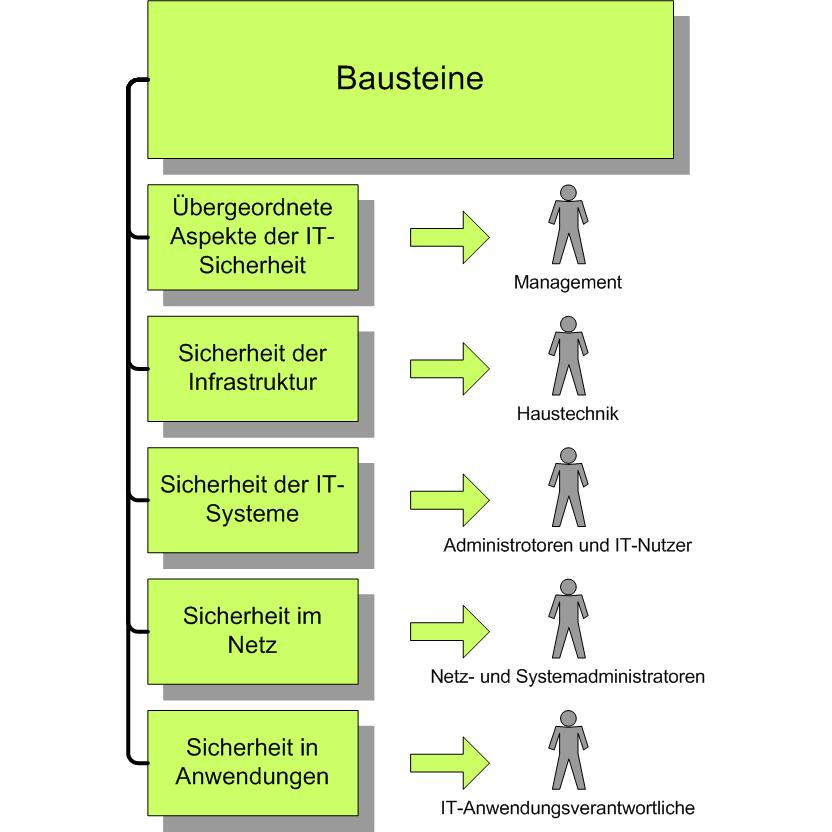
\includegraphics[width=0.8\textwidth,natwidth=832,natheight=832]{figures/Bausteinzuordnung_BSI_Grundschutzkataloge.jpg}
  		}
		\caption[Bausteinzuordnung-BSI-Grundschutzkataloge]{Bausteinzuordnung-BSI-Grundschutzkataloge}
		\label{Bausteinzuordnung-BSI-Grundschutzkataloge}
		\todo[inline]{Quelle Wikipedia hinzufügen}
	\end{figure}
	\pagebreak
	
	Die erste Schicht beschäftigt sich mit organisatorischen Fragen das Management, Personal oder Outsourcing betreffend. 
	In der Schicht Infrastruktur wird der Schwerpunkt auf bauliche Aspekte gelegt. 
	Die Schicht IT-Systeme befasst sich mit den Eigenschaften von IT-Systemen zu denen neben den Clients und Servern 
	auch Telefonanlagen oder Faxgeräte gezählt werden. In der Netze-Schicht werden Aspekte von Netzwerken beleuchtet. 
	Die Anwendungsschicht befasst sich mit Fragen sicherheitsrelevanter Software wie 
	Datenbankmanagementsystemen, E-Mail oder Webservern.
	Durch die Einteilung in Schichten lassen sich auch die von der jeweiligen Schicht 
	betroffenen Personengruppen klar eingrenzen. 
	Die erste Schicht spricht das Management an. Haustechniker sind von der zweiten betroffen. 
	Die dritte Schicht wird von Systemadministratoren abgedeckt. Die vierte Schicht fällt in den Aufgabenbereich der 
	Netzwerkadministratoren und die fünfte in den der Anwendungsadministratoren und der IT-Nutzer.
	Jeder einzelne Baustein folgt demselben Aufbau. Die Bausteinnummer setzt sich zusammen aus der Nummer 
	der Schicht in dem sich der Baustein befindet und einer in dieser Schicht eindeutigen Nummer. 
	Nach einer kurzen Beschreibung des vom Baustein betrachteten Sachverhalts wird die 
	jeweilige Gefährdungslage geschildert. 
	Anschließend folgt die Aufzählung der einzelnen Gefahrenquellen. 
	Diese stellen eine weiterführende Information dar und sind für die Erstellung eines Grundschutzes 
	nicht notwendigerweise durchzuarbeiten.

	Die notwendigen Maßnahmen werden mit kurzen Erläuterungen in einem Text vorgestellt. 
	Der Text folgt hierbei dem Lebenszyklus des jeweiligen Sachverhalts und umfasst 
	Planung und Konzeption, Beschaffung (falls erforderlich), Umsetzung, Betrieb, 
	Aussonderung (falls erforderlich) und Notfallvorsorge. 
	Nach der ausführlichen Schilderung werden die einzelnen Maßnahmen nochmals in einer Liste zusammengefasst, 
	die jedoch nun nach der Struktur der Maßnahmenkataloge und nicht mehr nach dem Lebenszyklus sortiert ist. 
	Hierbei wird eine Klassifizierung der Maßnahmen in die Kategorien A, B, C, Z und W vorgenommen. 
	Maßnahmen der Kategorie A bilden den Einstieg in die Thematik, B-Maßnahmen erweitern diese und die Kategorie C ist 
	anschließend notwendig für eine Zertifizierung des Grundschutzes. 
	Maßnahmen der Kategorie Z stellen zusätzliche Maßnahmen dar, die sich in der Praxis bewährt haben. 
	Maßnahmen der Kategorie W sind Maßnahmen die Hintergrundwissen zum jeweiligen Thema liefern 
	und für ein zusätzliches Grundverständnis der jeweiligen Thematik beitragen.
	\todo[inline]{Quelle Wikipedia hinzufügen}
	
	\begin{figure}[htbp]
		\centering
		\fbox{
    		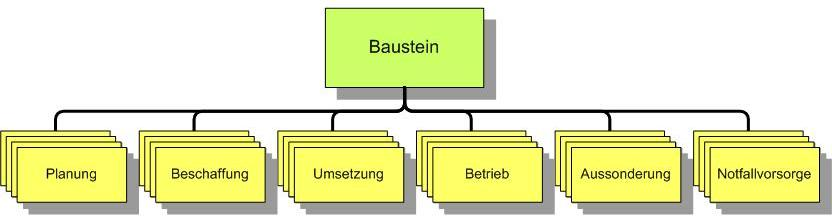
\includegraphics[width=0.8\textwidth,natwidth=832,natheight=218]{figures/Lebenszyklus_BSI_Grundschutzkataloge.jpg}
  		}
		\caption[Lebenszyklus-BSI-Grundschutzkataloge]{Lebenszyklus-BSI-Grundschutzkataloge}
		\label{Lebenszyklus-BSI-Grundschutzkataloge}
		\todo[inline]{Quelle Wikipedia hinzufügen}
	\end{figure}
	\pagebreak
 	
 	Des Weiteren finden sich Bausteine in Gefährdungskatalogen, welche verschiedene Gefährdungsszenarien 
 	beschreiben und wie folgst lauten:
 	
 	\begin{itemize}
 		\item G 1: Höhere Gewalt
 		\item G 2: Organisatorische Mängel
 		\item G 3: Menschliches Fehlverhalten
 		\item G 4: Technisches Versagen
 		\item G 5: Vorsätzliche Handlungen
 	\end{itemize}
 	Die Gefährdungskataloge gehen näher auf die möglichen Gefährdungen für IT-Systeme ein.
 	Diese Gefährdungskataloge folgen dem allgemeinen Aufbau nach Schichten.
 	Zur Erstellung des Grundschutzes ist nach Aussagen des BSI das in diesen Katalogen 
 	zusammengestellte Wissen nicht unbedingt notwendig, es fördert jedoch das Verständnis 
 	für die Maßnahme sowie die Wachsamkeit der Verantwortlichen. Die einzelne Gefahrenquelle 
 	ist in einem kurzen Text beschrieben und anschließend werden Beispiele für Schadensfälle, 
 	die durch diese Gefahrenquelle auslösen kann, gegeben.
 	\todo[inline]{Quelle hinzufügen}
 	\todo[inline]{Quelle=Wikipedia hinzufügen}
 	
 	Welche Maßnahmen und Normen einzuhalten sich um das Sicherheitslevel zu erhöhen, beschreiben die 
 	nachfolgenden sechs Punkte in Maßnahmenkatalogen: 
 	\begin{itemize}
 		\item M 1: Infrastruktur
 		\item M 2: Organisation
 		\item M 3: Personal
 		\item M 4: Hardware und Software
 		\item M 5: Kommunikation
 		\item M 6: Notfallvorsorge
 	\end{itemize}
 	Die zur Umsetzung des Grundschutzes notwendigen Maßnahmen sind in 
 	Maßnahmenkatalogen zusammengefasst. So werden Maßnahmen, 
 	die für mehrere System-Komponenten angemessen sind, nur einmal zentral beschrieben.
 	Hierbei werden auch Schichten zur Strukturierung der einzelnen Maßnahmengruppen genutzt.
 	In der jeweiligen Maßnahmenbeschreibung sind zunächst Verantwortliche für die Initiierung und 
 	die Umsetzung der Maßnahme genannt. Es folgt eine ausführliche Beschreibung der Maßnahme. 
 	Abschließend werden Kontrollfragen zur korrekten Umsetzung genannt.
 	Bei der Umsetzung der Maßnahmen sollte zunächst überprüft werden, 
 	ob eine Anpassung dieser auf den jeweiligen Betrieb notwendig ist. 
 	Eine genaue Dokumentation solcher Anpassungen ist zur späteren Nachvollziehbarkeit sinnvoll. 
 	Am Ende der Maßnahmen gibt es seit der 10. Ergänzungslieferung sogenannte Prüffragen, 
 	die die wesentlichen Aspekte einer Maßnahme nochmal aufgreifen und somit eine Art Checkliste darstellen,
 	ob diese auch umgesetzt sind.
 	\todo[inline]{Quelle=Wikipedia hinzufügen}
 	\todo[inline]{Quelle hinzufügen}
 	
 	Weiters gibt der IT-Grundschutzkatalog \todo[inline]{Quelle hinzufügen} wertvolle Hinweise, 
 	um theoretisch und praktisch einen effektiven Sicherheitsprozess zu gewährleisten.
 %\end{section}

 \pagebreak
 \label{Firewalls}
 \begin{section}{Firewalls}
	Das BSI hat sicherheitsspezifische Aspekte für Firewalls beschrieben.
	Sicherheitsspezifische Funktionen sind alle Funktionen einer Firewall, 
	die direkt zum Erreichen der Sicherheitsziele beitragen. \\
	
	Sicherheitsrelevante Funktionen tragen zum sicheren Funktionieren der Firewall 
	bei und leisten häufig nicht nur Dienste für die sicherheitsspezifischen Funktionen, 
	sondern auch für nicht sicherheitsbezogene Funktionen. Für gewöhnlich hängen 
	sicherheitsspezifische Funktionen vom korrekten Betrieb der sicherheitsrelevanten Funktionen ab. 
	Sicherheitsrelevante Funktionen sind alle Bestandteile, die für die Ausführung der 
	sicherheitsspezifischen Funktionen benötigt werden, also z.B. 
	Teile des Betriebssystems wie Netzwerktreiber, Bibliotheksfunktionen o.Ä. 
	Sie müssen also auch gemäß der oben aufgeführten Evaluationsstufen geprüft werden, 
	wobei auch Wechselwirkungen zu berücksichtigen sind! 
	Zur Erreichung einer größtmöglichen Vereinfachung und Standardisierung sollten die 
	sicherheitsrelevanten Funktionen über eine kleine Anzahl von genau definierten Schnittstellen 
	angesprochen werden können.
	Die sicherheitsspezifischen Funktionen einer Firewall lassen sich wie folgt unterteilen:
	\begin{itemize}
		\item Funktionen zum Schutz gegen direkte Angriffe
		\item Funktionen zum Schutz des zu sichernden Netzes gegen Angriffe aus dem unsicheren Netz
	\end{itemize}
	\todo[inline]{Quelle hinzufügen}
	\pagebreak
	
  \label{Sicherheitsdienste einer Firewall}
  \begin{subsection}{Sicherheitsdienste einer Firewall}
  	Auf dem Firewall-System werden Sicherheitsmechanismen implementiert, die diesen Übergang 
  	sicher und beherrschbar machen. Dazu analysiert das Firewall-System die Kommunikationsdaten, 
  	kontrolliert die Kommunikationsbeziehungen und Kommunikationspartner, 
  	reglementiert die Kommunikation nach einer Sicherheitspolitik, protokolliert sicherheitsrelevante 
  	Ereignisse und alarmiert bei starken Verstößen den Security-Administrator. \\
  	Nachfolgende Grafik zeigt die exemplarische Einbindung einer Firewall in ein Netzwerk und die Platzierung einer Firewall.
  	
  	\begin{figure}[htbp]
		\centering
		\fbox{
    		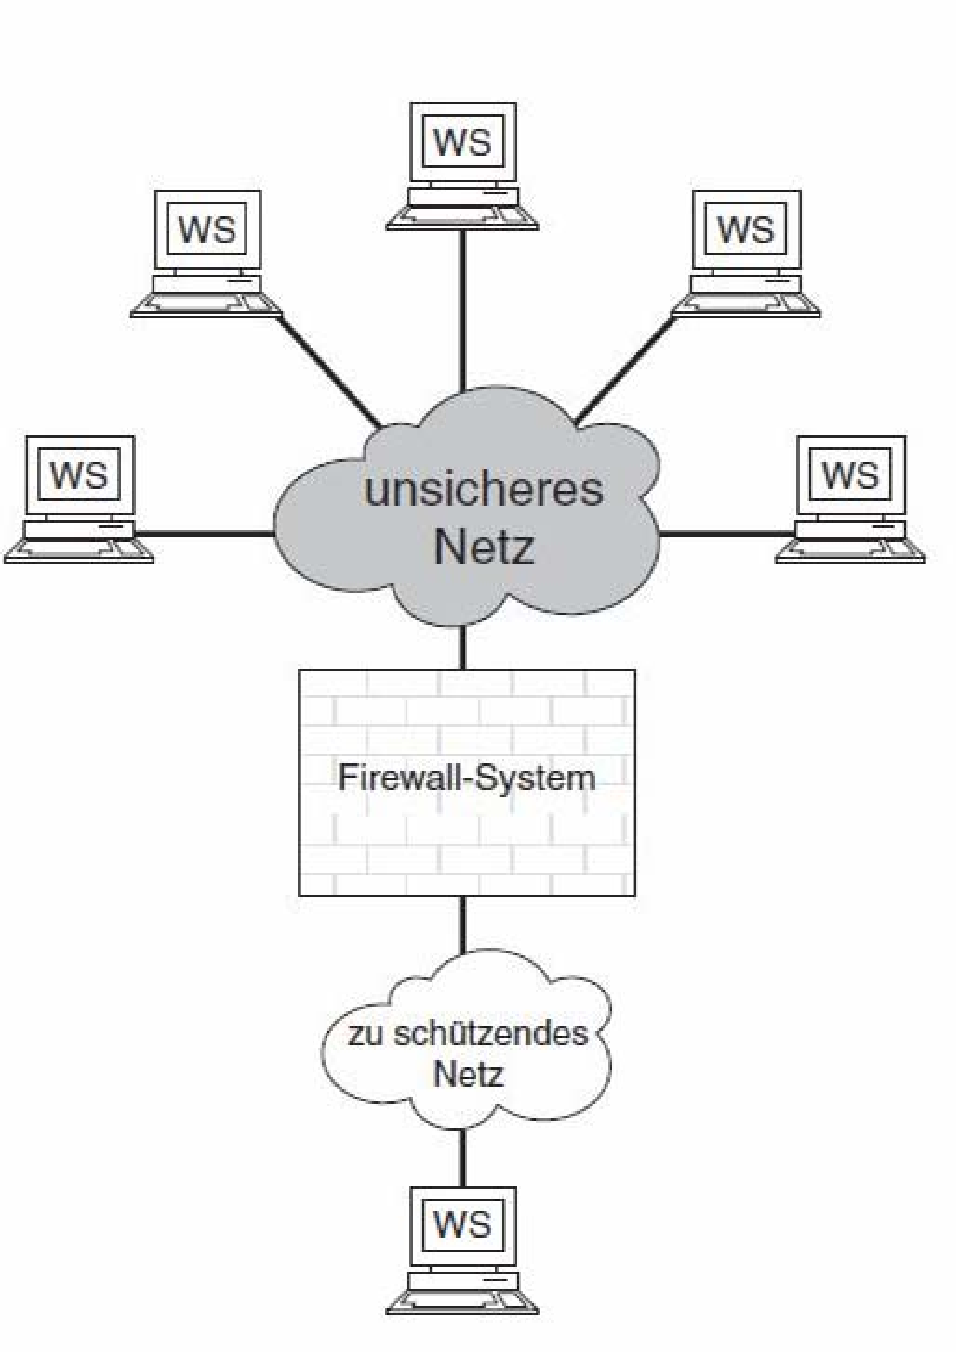
\includegraphics[width=0.8\textwidth,natwidth=514,natheight=556]{figures/Firewall_Nw.pdf}
    		%[height=60mm, width=100mm]
    		%\centering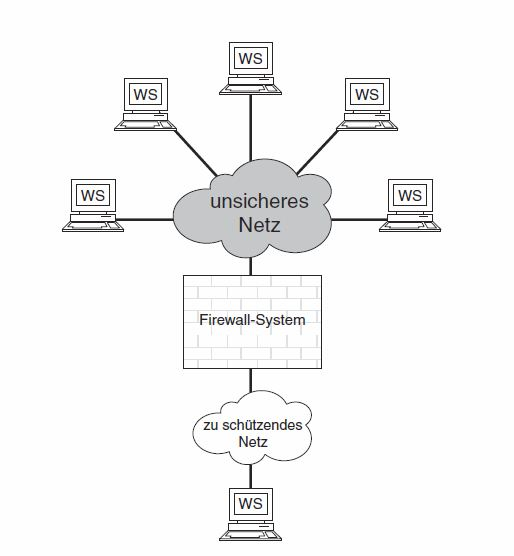
\includegraphics[scale=15%]{figures/Firewall_Nw.jpg}
  		}
		\caption[Firewall:Network]{Firewall-Network}
		\label{Firewall_Network}
		\todo[inline]{Quelle hinzufügen}
	\end{figure}
  \end{subsection}
  \pagebreak
  
  \label{Firewall-Konzepte}
  \begin{subsection}{Firewall-Konzepte}
  	Ein Firewall-System stellt den "Common Point of Trust" für den Übergang zwischen 
  	unterschiedlichen Netzen dar, d.h., der einzige Weg ins interne Netz führt kontrolliert über das Firewall-System.
  	\\
  	Firewall-Systeme werden verwendet, um sich an unsichere Netze wie z.B. das Internet anzukoppeln 
  	oder auch, um das eigene Netz zu strukturieren und hier 
  	Sicherheitsdomänen mit unterschiedlichem Schutzbedarf zu schaffen.
  	\todo[inline]{Quelle hinzufügen}
  	
  	\textbf{Vorteile des Common-Point-of-Trust-Konzeptes}
  	\begin{itemize}
  		\item Kosten:
  			Die Realisierung von Sicherheitsmechanismen auf einem zentralen System ist wesentlich einfacher jene 
  			auf jedem einzelnen Rechner.
  		\item Möglichkeiten durch Sicherheitspolitik:
  			Durch eine zentrale Steuerung können die Benutzer einheitlich authentifiziert werden und womöglich 
  			mit kryptographischen Funktionen erweitert werden.
  		\item Abschottung:
  			Durch diese Konzeptionierung kann das zu schützende Netzwerk von unsicheren Netzwerken getrennt werden.
  			Firewall-Systeme können Angriffen entgegenwirken.
  	\end{itemize}
  	\todo[inline]{Quelle hinzufügen}
  	
  	\textbf{Allgemeine Ziele von Firewall-Systemen}
  	\begin{itemize}
  		\item Zugangskontrolle:
  			Auf Daten-, Benutzer- und Netzwerkebene kann die Sicherheit überprüft und gewährleistet werden, 
  			damit ein sicherer Datenaustausch möglich ist.
  		\item Rechteverwaltung:
  			Mittels Protokollen und Diensten kannst festgelegt werden, wann für wen eine Kommunikation über das 
  			Firewall-System erlaubt ist.
  		\item Vertraulichkeit:
  			Die interne Struktur wird hinter dem Schutzsystem verborgen und Nachrichten werden nie im Klartext 
  			übermittelt.
  	\end{itemize}
  	\todo[inline]{Quelle hinzufügen}
  \end{subsection}
 \end{section}
\pagebreak


%%%%%%%%%%%%%%%%%%%%%%%%%%%%%%%%%%%%%%%%%
\chapter{Grundlagen von VoIP}
\label{ch:ch3}
%%%%%%%%%%%%%%%%%%%%%%%%%%%%%%%%%%%%%%%%%
\label{Grundlagen von VoIP}
% \begin{section}{Grundlagen von VoIP}
	Allgemein gesprochen beschreibt Voice over IP die Telefonie basierend auf dem \ac{TCP/IP} Protokoll im Internet.
	
	Mit VoIP werden mehrere Begriffe verbunden; z.B.:
	\begin{itemize}
		\item \ac{IP}-Telefonie
		\item Skype
		\item \ac{LAN}-Telefonie
		\item \ac{SIP}-Telefonie
		\item Internettelefonie
	\end{itemize}

 \label{Geschichte der Telefonie}
 \begin{section}{Geschichte der Telefonie}
 	Kommunikation ist ein Grundbedürfnis aller Menschen. Allein wie die Information übermittelt wird, 
 	hat sich im Laufe der Geschichte immer wieder geändert. 
 	Seit Jahrzehnten ist das Telefon fester Bestandteil unseres Lebens. 
 	Der Griff zum Hörer, der Gespräche mit Menschen rund um die Welt ermöglicht, 
 	ist heute eine Selbstverständlichkeit. Vor 12 Jahren, 
 	als die Geschichte der Telefonie in Österreich begann, war das Telefon jedoch eine sensationelle Innovation. \\
 	\\
 	Im Juni des Jahres 1881 erteilte das k.k. Handelsministerium der "Wiener Privat-Telegraphen-Gesellschaft" 
 	eine "Concession" zum Betrieb von Telefonanlagen. Zwar erscheint die Netzabdeckung aus 
 	heutiger Sicht wenig beeindruckend, die Telefonanlagen durften lediglich in einem Umkreis 
 	von 15 Kilometern rund um den Wiener "Stephansthurm" betrieben werden. 
 	Schon drei Monate später wurde der Betrieb der Telefonanlagen auf ganz Wien ausgeweitet, 
 	im Dezember 1881 konnte in der Wiener Friedrichstraße die erste Telefonzentrale Österreichs 
 	eröffnet werden. Mit 154 Teilnehmern, darunter Zeitungen, Großunternehmer und Banken, 
 	wurde der Netzbetrieb gestartet. \\
 	\\
 	Im Jahr 1867 entwickelte Alexander Graham Bell eine Versuchsanordnung, 
 	bei der Schallwellen der menschlichen Sprache eine Membran vibrieren ließen. 
 	Dadurch entstanden in einer Drahtspule Stromschwankungen, 
 	die nach der Übertragung auf ein gleichartiges Gerät wieder Töne hervorbrachten. 
 	Bell erhielt für seine Erfindung die Patentnummer 174.465 und war damit nur um zwei Stunden 
 	schneller als der Amerikaner Elisha Gray. Damals konnte noch niemand ahnen, 
 	dass die Erfindung zu einem der einträglichsten Patente aller Zeiten werden sollte. 
 	Im Jahr 1876 wurde über den "Bellschen Sprachtelegraphen" schließlich zwischen 
 	Boston und Cambridge das erste Ferngespräch der Welt geführt.
 	\pagebreak
 	
 	Im Jahre 1910 kamen schließlich die ersten Telefone, die mit einer Wählscheibe und 
 	einem Hörer ausgestattet waren, auf den Markt. Zugleich bereitete die 
 	Post- und Telegraphenverwaltung mit der Umstellung der Verbindungen innerhalb eines Ortes 
 	vom handvermittelten Dienst auf Selbstwählverkehr eine kleine Revolution vor. 
 	Nun konnten die Teilnehmer erstmals ihre Gesprächspartner innerhalb eines Ortes 
 	direkt und ohne Vermittlungshilfe erreichen. Schon in den Anfangsjahren der Telefonie 
 	gab es Verbindungen in die österreichischen Kronländer. Allerdings wurden diese Leitungen 
 	bis etwa 1920 ausnahmslos über Freileitungstrassen geführt. \\

 	\cite{stadtwien2012Telefon}
 	\pagebreak
 \end{section}
 
 \label{Einführung in VoIP}
 \begin{section}{Einführung in VoIP}
 	Mit der Thematik Voice over IP hat die Telefonie einen riesen Schritt vorwärts getan.
 	Durch die starke Verbreitung von Smartphones haben sich noch weitere Geschäftsfelder für 
 	die Internettelefonie hinzugekommen. Internationale Firmen haben diese Chancen längst erkannt 
 	und stellen sich dementsprechend auf. \\
 	Basierend auf den Protokollen \ac{IP}, \ac{TCP} und \ac{UDP} lässt sich VoIP leicht in bestehende 
 	Infrastruktur und Dienste integrieren.
 	Im nächsten Kapitel werden die technischen Details noch näher erläutert. \\
 	Firmen nutzen die gleiche Infrastruktur zur Datenübertragung und zur Telefonie.
 	Das brachte viele Vorteile mit sich und somit auch den Durchbruch für VoIP.
 	Herkömmliche Telefonie war davor immer kanalorientiert gewesen. 
 	Im Bereich von VoIP spricht man von einer Paketorientierung im Bezug 
 	auf die Verbindung. \\
	Eine paketorientierte Übertragung von Sprache nutzt Leitungskapazität 
	gezielter aus als die bisherige Methode einer Reservierung der gesamten Leitung.
	Durch Effizienz in der Mediumsnutzung und Flexibilität in der Anwendung ergab sich 
	im Laufe der Zeit eine Überlegenheit von VoIP. \\
	\todo[inline]{Quelle hinzufügen}
	Als Konsequenz daraus ergibt sich eine hohe Erreichbarkeit.
	Gebremst werden kann das nur durch die verfügbare Bandbreite, welche sich 
	aber im Laufe der letzten Jahre verbessert hat. Das aufkommende Datenvolumen 
	spielt in seltenen Fällen eine Rolle - wird jedoch von den Providern kritischer 
	gesehen. \\
	Wesentlich für das Zustandekommen von Internettelefonie und Gesprächen ist, 
	dass die analoge Telefonie digital verarbeitet wird. 
	Die Sprache wird in IP-Pakete umgewandelt und in manchen Fällen auch verschlüsselt, 
	um die Sicherheit zu erhöhen.
	
 	\todo[inline]{Quelle hinzufügen}
 	
 	\textbf{Vorteile von VoIP}
 	\begin{itemize}
 		\item Interne Gespräche ohne Gebühren
 		\item Daten und Sprachübertragung in einem Medium
 		\item Ortsungebundenheit im Gegensatz zum Festnetz
 		\item Kostenersparnis bei Auslandsgesprächen
 		\item Erweiterbarkeit
 		\item Unabhängige Komplettlösung
 	\end{itemize}
 	
 	\textbf{Nachteile von VoIP}
 	\begin{itemize}
 		\item Sicherheitsrisiko durch Abhängigkeit von Internet
 		\item Qualitätsdefizit möglicherweise durch Hardware und Bandbreite
 		\item Zuverlässigkeit fraglich durch Hardwaredefekt oder Leitungsausfall
 		\item Notrufe nur eingeschränkt möglich
 		\item Stromkosten wesentlich höher
 		\item Externe Abhängigkeit von regionaler Infrastruktur (z.B. Stromnetz)
 	\end{itemize}
 	\todo[inline]{Quelle hinzufügen}
 	 	
 \end{section}
 
 \label{Technische Grundlagen einer VoIP-Infrastruktur}
 \begin{section}{Technische Grundlagen einer VoIP-Infrastruktur}
	Bei der Internettelefonie gibt es mehrere Schwerpunkte, die in diesem Kapitel 
	diskutiert werden.
	Die Kernfragen sind der Transport der Sprache, die Sicherung von Datenströmen 
	und Sprachinformationen und der Medienübergang in angrenzende Systeme.
 	\label{Protokolle und Standards}
 	\begin{subsection}{Protokolle und Standards}
 		\todo[inline]{RTP und RTCP}
 		\todo[inline]{H.323}
 		\todo[inline]{SIP}
 		\todo[inline]{SIP - STP}
 	\end{subsection}
 
 	\label{Anforderungen an die technische Infrastruktur}
 	\begin{subsection}{Anforderungen an die technische Infrastruktur}
 	\end{subsection}
 
	 \label{Komponenten}
 	\begin{subsection}{Komponenten}
 	\end{subsection}
 
 \end{section}
 
 \label{Fallbeispiel: Exemplarischer Aufbau einer VoIP-Infrastruktur}
 \begin{section}{Fallbeispiel: Exemplarischer Aufbau einer VoIP-Infrastruktur}
 \end{section}
 
% \end{section}


%%%%%%%%%%%%%%%%%%%%%%%%%%%%%%%%%%%%%%%%%
\chapter{Angriffe auf VoIP}
\label{ch:ch4}
%%%%%%%%%%%%%%%%%%%%%%%%%%%%%%%%%%%%%%%%%
\label{Angriffe auf VoIP}
%\begin{section}{Angriffe auf VoIP}

 \label{Überblick über die häufigsten Sicherheitsprobleme}
 \begin{section}{Überblick über die häufigsten Sicherheitsprobleme}
 \end{section}
 
 \label{Detaillierte Angriffsschemata}
 \begin{section}{Detaillierte Angriffsschemata}
 \end{section}
 
 \label{IP-basierte Schwachstellen}
 \begin{subsection}{IP-basierte Schwachstellen}

  \begin{subsubsection}{DoS}
  \end{subsubsection}
  \begin{subsubsection}{Flooding}
  \end{subsubsection}
  \begin{subsubsection}{Umleitungen}
  \end{subsubsection}
  \begin{subsubsection}{Datenmanipulation}
  \end{subsubsection}  
  
 \end{subsection}
 
 \label{Weitere Schwachstellen}
 \begin{subsection}{Weitere Schwachstellen}
   
  \begin{subsubsection}{Eavesdropping}
  \end{subsubsection}
  \begin{subsubsection}{ARP-Poisoning}
  \end{subsubsection}
  \begin{subsubsection}{SIP Proxy Angriffe}
  \end{subsubsection}
  \begin{subsubsection}{SIP Phone Angriffe}
  \end{subsubsection}
  \begin{subsubsection}{VoIP-Phishing}
  \end{subsubsection}
  
 \end{subsection}
 
 \label{Tools für den Angriff auf VoIP}
 \begin{section}{Tools für den Angriff auf VoIP}
 \end{section}
 
%\end{section}


%%%%%%%%%%%%%%%%%%%%%%%%%%%%%%%%%%%%%%%%%
\chapter{Erhöhung der Sicherheit durch VoIP-Firewalls}
\label{ch:ch5}
%%%%%%%%%%%%%%%%%%%%%%%%%%%%%%%%%%%%%%%%%
\label{Erhöhung der Sicherheit durch VoIP-Firewalls}

 \label{Funktionen}
 \begin{section}{Funktionen}
 \end{section}
 
 \label{Aufbau und Spezifikationen}
 \begin{section}{Aufbau und Spezifikationen}
 \end{section}


%%%%%%%%%%%%%%%%%%%%%%%%%%%%%%%%%%%%%%%%%
\chapter{Conclusio und Ausblick}
\label{ch:ch7}
%%%%%%%%%%%%%%%%%%%%%%%%%%%%%%%%%%%%%%%%%
\label{Conclusio und Ausblick}


%%%%%%%
%%%%%%%%%%%%%%%%%%%%%%%%%%%%%%%%%%%%%%%%%%%%%%%%%%%%%%%%%%%%%%%%%%%%%%%%
\chapter{Ergebnisse}
\label{sec:results}
%%%%%%%%%%%%%%%%%%%%%%%%%%%%%%%%%%%%%%%%%%%%%%%%%%%%%%%%%%%%%%%%%%%%%%%%

Die Resultate der Arbeit präsentieren und nach Möglichkeit aussagekräftige, eigenständige Abbildungen einbauen. Namen des Kapitels konkretisieren, an jeweilige Arbeit anpassen -- Lösungsvorschlag/Implementierung im Titel des Kapitels benennen. Bei einer Software-Entwicklungsarbeit ggf. eine Beschreibung der Qualitätsmerkmale der neuen Implementierung (Performance, Sicherheit, Messergebnisse etc.) geben.

Bei einer Arbeit zu einem abstrakteren Architekturthema können hier die Eigenschaften nach der Anwendung der konzipierten Architektur beschrieben werden. Kommt sie in mehreren Fallbeispielen zum Einsatz, erfolgt hier ein Vergleich der jeweiligen Ergebnisse (z.B. gab es Unterschiede im Umsetzungserfolg, die sich auf konkrete Eigenschaften der betrachteten Fallbeispiele zurückführen lassen).

Bei einer Arbeit zur Softwareauswahl und Einführung wird eine Beschreibung von Qualitätseigenschaften des mit der Einführung neu geschaffenen SOLL-Zustands gegeben.

Bei einer Arbeit, deren Fokus auf der Durchführung und Auswertung von Fragebögen liegt, erfolgt in diesem Kapitel die Auswertung der Fragebögen.
%%%%%%%%%%%%%%%%%%%%%%%%%%%%%%%%%%%%%%%%%%%%%%%%%%%%%%%%%%%%%%%%%%%%%%%%
\chapter{Zusammenfassung und Ausblick}
\label{sec:conclusion}
%%%%%%%%%%%%%%%%%%%%%%%%%%%%%%%%%%%%%%%%%%%%%%%%%%%%%%%%%%%%%%%%%%%%%%%%

Die Zusammenfassung ist nach der Kurzfassung der am häufigsten gelesene Teil, da viele Leser aus Zeitknappheit Arbeiten im Schnellverfahren konsumieren und rasch zur Zusammenfassung blättern. Hier hat man die Chance, dem Leser noch einmal die zentralen Ideen und Ergebnisse der Diplomarbeit zu vermitteln.

Im Gegensatz zur Kurzfassung sind die Leser mit der Problemstellung und der Terminologie bereits vertraut. In der Länge hat man deutlich mehr Spielraum als bei der Kurzfassung, die Zusammenfassung sollte inklusive Ausblick 2 bis max. 10 Seiten umfassen. Hier sollten kompakt die Antworten auf die in der Zielsetzung aufgeworfenen Fragen (Hypothesen) gegeben werden.

Neben einer Zusammenfassung der wichtigsten Ergebnisse sollte auch ein Ausblick gegeben werden: Aufzeigen des Bedarfs an zukünftiger Forschung, potentielle Anwendungsmöglichkeiten der vorgestellten Lösung etc.

In Summe sollte die Zusammenfassung dem Leser die wissenschaftliche und, wenn vorhanden, praktische Relevanz der Arbeit klar und verständlich darlegen.

% insert bibliography and such stuff
\BackMatter

\cleardoublepage
\appendix

%%%%%%%%%%%%%%%%%%%%%%%%%%%%%%%%%%%%%%%%%%%%%%%%%%%%%%%%%%%%%%%%%%%%%%%%
\chapter{\appendixlabel}
%%%%%%%%%%%%%%%%%%%%%%%%%%%%%%%%%%%%%%%%%%%%%%%%%%%%%%%%%%%%%%%%%%%%%%%%

\whichlanguage{
Listings, data models, forms, \dots
}{
Quellcode, Datenmodell, Fragebögen, \dots
}
%\chapter{Hinweise zur Literatur}
\label{sec:references}

\section{Literatursuche}

Informationen zu Onlinebibliotheken und Literatursuche, z.B. Magazine, Jounals, Konferenzen und Organisationen können unter \url{http://www.big.tuwien.ac.at/teaching/info.html} gefunden werden.

\section{BibLatex}

Biblatex beitet verschiedene Möglichkeiten an um Literatur zu referenzieren. Die beiden häufigsten Befehle sind \verb|\cite| und \verb|\citeauthor|.

Beispiele wie referenziert werden kann:\\
\citeauthor{fankhauser:2009:softwaretechnik-security} beschreiben in \cite{fankhauser:2009:softwaretechnik-security} \dots\\
In \cite{schanes:2011:voip-fuzzer} zeigt \citeauthor{schanes:2011:voip-fuzzer} wie \dots
Weitere Informationen können von \cite{oasis:2010:homepage} in \cite{oasis:2010:homepage} entnommen werden.

Wir empfehlen JabRef um die Literaturdatenbank zu verwalten.

% \chapter{}
% 
% \section{Literature Search}
% 
% Information on online libraries and literature search, e.g., interesting magazines, journals, conferences, and organizations may be found at \url{http://www.big.tuwien.ac.at/teaching/info.html}.
% 
% \section{BibTeX}
% 
% BibTeX should be used for referencing.
% 
% The LaTeX source document of this pdf document provides you with different samples for references to journals~\cite{jour:B2BServices}, conference papers~\cite{proc:TheWebMLApproach}, books~\cite{book:umlatwork}, book chapters~\cite{incoll:ErhardKonrad1992}, electronic standards~\cite{man:BPEL}, dissertations~\cite{phdthesis:manuelWimmer}, masters' theses~\cite{mast:AUMLProfile}, and web sites~\cite{BIGWebsite}. The respective BibTeX entries may be found in the file \texttt{references.bib}. For administration of the BibTeX references we recommend \url{http://www.citeulike.org} or JabRef for offline administration, respectively.

%\chapter{Algorithmen und Quellcode}

\section{Beispiele für Quellcode}

Beispiel eines Quellcodes ist im Quellcode \ref{lst:shortcode} zu finden.

\begin{lstlisting}[caption={Short code},label=lst:shortcode]
//Start Program
System.out.println("Hello World!");
//End Program
\end{lstlisting}


\section{Beispiele für Algorithmen}

Algorithmus \ref{alg:samplealgorithm} dient als Beispiel.

\begin{algorithm}[t]
\SetKwData{Left}{left}
\SetKwData{This}{this}
\SetKwData{Up}{up}
\SetKwFunction{Union}{Union}
\SetKwFunction{FindCompress}{FindCompress}
\SetKwInOut{Input}{input}
\SetKwInOut{Output}{output}

\Input{A bitmap $Im$ of size $w\times l$}
\Output{A partition of the bitmap}

\BlankLine

\emph{special treatment of the first line}\;
\For{$i\leftarrow 2$ \KwTo $l$}{
\emph{special treatment of the first element of line $i$}\;
\For{$j\leftarrow 2$ \KwTo $w$}{\label{forins}
\Left$\leftarrow$ \FindCompress{$Im[i,j-1]$}\;
\Up$\leftarrow$ \FindCompress{$Im[i-1,]$}\;
\This$\leftarrow$ \FindCompress{$Im[i,j]$}\;
\If(\tcp*[r]{O(\Left,\This)==1}){\Left compatible with \This}{\label{lt}
\lIf{\Left $<$ \This}{\Union{\Left,\This}}\;
\lElse{\Union{\This,\Left}\;}
}
\If(\tcp*[r]{O(\Up,\This)==1}){\Up compatible with \This}{\label{ut}
\lIf{\Up $<$ \This}{\Union{\Up,\This}}\;
\tcp{\This is put under \Up to keep tree as flat as possible}\label{cmt}
\lElse{\Union{\This,\Up}}\tcp*[r]{\This linked to \Up}\label{lelse}
}
}
\lForEach{element $e$ of the line $i$}{\FindCompress{p}}
}
\caption{Sample algorithm}\label{alg:samplealgorithm}
\end{algorithm}


\end{document}
